\documentclass[10pt]{extarticle}

\usepackage[utf8]{inputenc}              % Tipos de caracteres
\usepackage[portuguese]{babel}           % Português
\usepackage[a4paper,portrait]{geometry}  % Tipo de papel
\usepackage{color}                       % Para tratamento da cor
\usepackage{graphicx}                    % Para a imagem
\DeclareGraphicsExtensions{.jpg,.png}
\usepackage{amsmath}                     % Para as matematiquices
\usepackage{amssymb}
\usepackage{array}
\usepackage{gensymb}                     % Grau
\usepackage{multicol}
\setlength{\columnsep}{1cm}
\usepackage{geometry}					% Margens
%\usepackage{xfrac}
%\usepackage{colortbl}

\usepackage{multirow}

\addtolength{\topmargin}{-20mm}
\addtolength{\textheight}{50mm}
\addtolength{\oddsidemargin}{-15mm}
\addtolength{\textwidth}{32mm}

\renewenvironment{abstract}
 {\small
  \begin{center}
  \bfseries \abstractname\vspace{-.5em}\vspace{0pt}
  \end{center}
  \list{}{
    \setlength{\leftmargin}{0cm}%
    \setlength{\rightmargin}{\leftmargin}%
  }%
  \item\relax}
 {\endlist}
 
\renewcommand{\abstractname}{Resumo}

\delimitershortfall-1sp
\newcommand\abs[1]{\left|#1\right|}
\newcommand{\PR}[1]{\ensuremath{\left[#1\right]}}
\newcommand{\PC}[1]{\ensuremath{\left(#1\right)}}
\newcommand{\chav}[1]{\ensuremath{\left\{#1\right\}}}

\newcolumntype{x}[1]{>{\centering\hspace{0pt}}p{#1}}

\begin{document}

\title {\bf \huge T0 - Caracterização de uma Célula Fotovoltaica}
\author
{{\small Grupo III - João Ferreira (78179) Henrique Rodrigues (78632) Rodrigo C. Carvalho (78646) Cristina Melício (78947)} \\
{\small MEFT - 2ºAno, 2º Semestre - Laboratório de Complementos de Eletromagnetismo e Termodinâmica}}
\date{{\small Sexta-Feira, 27 de Fevereiro de 2014}}
\maketitle

\begin{multicols}{2}

\section{Introdução}

O conversor termoelétrico é um dispositivo que permite criar uma diferença de potencial a partir de uma diferença de temperaturas, e vice-versa. 

Os fenómenos que estão na explicação desta experiência são o efeito de \textit{Seeback}, de \textit{Peltier} e de \textit{Thomson}. O efeito de \textit{Seeback}, consiste em impor uma diferença de temperaturas entre as placas condutoras nas extremidades da célula, $\Delta T$, de modo a obter uma diferença de potencial, $V$, estando estas relacionadas pelo coeficiente de \textit{Seeback}:
\begin{equation}
S_{A,B} = \frac{V}{\Delta T}
\end{equation}
onde A e B correspondem aos materiais das extremidades. Já o efeito de \textit{Peltier} consiste em impor uma diferença de potencial á célula de modo a produzir um gradiente de temperatura entre as placas, estando a densidade de fluxo de calor, $J_Q$, relacionado com a corrente por unidade de área, J, pelo coeficiente de \textit{Peltier}:
\begin{equation}
\Pi_{A,B} = \frac{J_{Q_{A}}-J_{Q_{B}}}{J}
\end{equation}
A relação que se estabelece entre estes dois efeitos é conhecida pela Segunda Relação de Kelvin e é dada por:
\begin{equation}
\Pi_{A,B} = T S_{A,B}
\end{equation}
Considera-se ainda o efeito de \textit{Thomson} se exixtir grandiente do coeficiente de Seeback, ou seja, se não depender linearmente com a temperatura. Sendo assim, o coeficiente de \textit{Thomson} é dado por:
\begin{equation}
\tau = \frac{\dot{q}_{Thomson}}{\vec{J} \cdot \vec{\nabla} T}
\end{equation}
A relação dada pelos três efeitos, Primeira Relação de Kelvin, corresponde a:
\begin{equation}
\frac{d \Pi_{A,B}}{dT} + \tau_A - \tau_B = S_{A,B}
\end{equation}
Nesta experiência o conversor termoelétrico tem por base uma célula de \textit{Peltier} em contacto com duas placas condutoras de metais diferentes.

Na primeira parte o mecanismo, cujo esquema está representado na figura 1, é usado como máquina térmica, pelo que o seu rendimento é dado por:
\begin{equation}
\eta_1=\frac{P_2}{P_{E_{1}}}
\end{equation}
onde $P_2$ e $P_{E_{1}}$ são, respetivamente, a potência dissipada na resistência $R_2$ (ligada à célula) e a potência fornecida pela fonte quente $E_1$, dadas pelas seguintes expressões:
\begin{gather}
P_{E_{1}} = V_1 I_1 \\
P_2 = \frac{{V_2^2}}{R_{2_{0}}}
\end{gather}

\hspace{-0.8cm}
\begin{center}
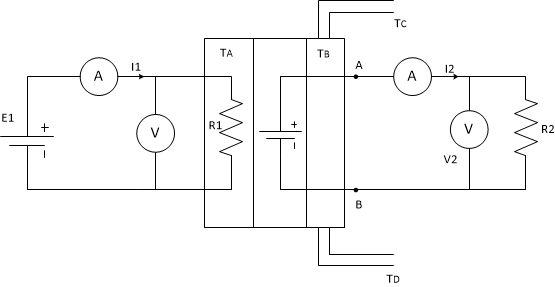
\includegraphics[width=220pt]{figura1.png}
\begin{center}
\par\noindent {\scriptsize (Figura 1: Esquema da montagem)}
\end{center}
\end{center}

Para maximizar o rendimento determina-se a resistência de carga ótima, $R_{2{_0}}$ para a qual a potência $P_2$ é máxima dada pela fórmula:
\begin{equation}
R_{2{_0}} = 5I_{2{_5}} - 2I_{2{_2}} - 2 R_a
\end{equation}
onde $R_a$ é a resistência interna do amperímetro obtida pela fórmula:
\begin{equation}
R_a = \frac{V_a}{I_2} 
\end{equation}

Uma vez que existem perdas de energia, nem toda a potência fornecida pela fonte quente chega à fonte fria ou é transformada pela célula em corrente, sendo necessário considerar também a potência retirada da fonte fria pelo fluido de arrefecimento, ou seja, $ P_3$ que se obtém com seguinte equação:
\begin{equation}
P_3 = \frac{\Delta m}{\Delta t} C (T_c-T_d)
\end{equation}

Como $P_1 > P_2 + P_3$, tem-se a primeira correção ao rendimento:
\begin{equation}
\eta_2=\frac{P_2}{P_2+P_3}
\end{equation}
Para a última correção ao rendimento considera-se ainda que uma parte da potência passa da fonte quente para a fonte fria por condução através da célula fotovoltaica, obtendo a fórmula:
\begin{equation}
\eta_3=\frac{P_2}{P_2+P_3-P_{3_{conducao}}}
\end{equation}
De forma a calcular a potência dissipada por condução considera-se uma resistência térmica entre a fonte fria $T_A$ e a quente $T_B$, cuja formula é:
\begin{equation}
R_T = \frac{T_A - T_B}{P_3}
\end{equation}
Para avaliar o desempenho da máquina tem-se como referência o rendimento do motor reversível operando entre as temperaturas das fontes.
\begin{equation}
\eta_{Carnot} = 1 - \frac{T_B}{T_A}
\end{equation}

Na segunda parte da experiência, com base no efeito de \textit{Peltier}, o conversor, representado na figura 2, é utilizado como bomba de calor, sendo a eficiência determinada pela expressão:
\begin{equation}
\varepsilon=\frac{P_3}{P_{E_{2}}}
\end{equation}
em que $P_{E{_2}}$ é a potência cedida pela fonte de tensão $E_2$ e é dada pela expressão:
\begin{equation}
P_{E_{2}}= V_2 I_2
\end{equation}

\hspace{-0.8cm}
\begin{center}
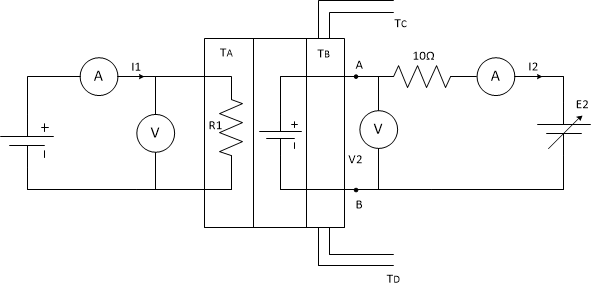
\includegraphics[width=220pt]{figura2.png}
\begin{center}
\par\noindent {\scriptsize (Figura 1: Esquema da montagem)}
\end{center}
\end{center}

A eficiência de referência é a da máquina de Carnot, cuja temperatura da fonte quente é $T_A$, e da fonte fria $T_B$, dada pela expressão:
\begin{equation}
\varepsilon_{Carnot} = \frac{T_B}{T_B - T_A}
\end{equation}

\newpage
%\section{Introdução}

%\par 

%\begin{equation} \label{eq:1}
%\gamma = \frac{1}{\sqrt{1-\frac{v^2}{c^2}}}
%\end{equation}

%\begin{center}
%\par\noindent {\scriptsize (onde ...)}
%\end{center}

%\section{Procedimento Experimental}

%\begin{center}
%\includegraphics[width=240pt]{ftg9}
%\end{center}

%\begin{center}
%\begin{tabular}{ x{0.4cm} x{1.1cm} x{1.1cm} x{1.1cm} x{1.1cm} }
%i & $p_x$ & $\varepsilon_{p_x}$ & $p_y$ & $\varepsilon_{p_y}$ \tabularnewline 
% & {\scriptsize $(MeV/c)$} & {\scriptsize $(MeV/c)$} & {\scriptsize $(MeV/c)$} & {\scriptsize $(MeV/c)$} \tabularnewline 
%\hline \hline
%\multicolumn{5}{x{6.5cm}}{Método 1} \tabularnewline
%\hline \hline
%1      & -2033 & -   & 0    & -  \tabularnewline
%3      & 766   & 68  & 383  & 31 \tabularnewline
%4      & 291   & 34  & -430 & 45 \tabularnewline
%$\sum$ & -976  & 102 & -47  & 75 \tabularnewline
%\hline \hline
%\multicolumn{5}{x{6.5cm}}{Método 2} \tabularnewline
%\hline \hline
%1      & -2033 & -  & 0    & -  \tabularnewline
%3      & 775   & 68 & 395  & 40 \tabularnewline
%4      & 306   & 30 & -437 & 42 \tabularnewline
%$\sum$ & -952  & 98 & -43  & 81 \tabularnewline
%\end{tabular}
%\end{center}

%\begin{center}
%\par\noindent {\scriptsize (Tabela 3: Momentos lineares e seu balanço, referentes à colisão da fotografia 9)}
%\end{center}

%\section{Análise de Resultados e Conclusões}

%\par 

%\vfill

%\pagebreak

%\section{Anexos}

%\subsection*{\normalsize Material}

%\begin{itemize}
%\item D
%\end{itemize}

%\subsection*{\normalsize Tabelas Completas de Resultados}

%\begin{center}
%\begin{tabular}{ x{2cm} x{2cm} x{2cm} }
%Partícula & $m$ {\scriptsize $(MeV/c^2)$} & $q/q_{p^+}$
% \tabularnewline
%\hline \hline
%$p^+$   & $938$ & 1 \tabularnewline
%$n^0$   & $939$ & 0 \tabularnewline
%$\pi^0$ & $135$ & 0 \tabularnewline
%$\pi^+$ & $140$ & 1 \tabularnewline
%\end{tabular}
%\end{center}

%\begin{center}
%\par\noindent {\scriptsize (Tabela 1A: Massa e carga das partículas analisadas)}
%\end{center}

%\subsection*{\normalsize Fórmulas de Erro}

%\begin{equation}
%\varepsilon_{p_{col}}=\frac{E_i}{c^2p_{col}}\varepsilon_l
%\end{equation}

\end{multicols}

\end{document}